The retinal model described in section \ref{sec-fov-pit} is
parallel in nature it involves changing each pixel locally.
Convolution kernels are computed and stored in memory prior 
to any convolution procedure. OpenCL is used since 
the same code can be used in multiple Operating Systems (OS) 
and hardware targets \cite{munshi2011opencl}.

\subsection{Na\"{i}ve approach}
\begin{wrapfigure}{r}{0.55\textwidth}
    \vspace{-26pt}
    \begin{minipage}{0.55\textwidth}
        \begin{pseudocode}{Na\"ive convolution}{image \; I,\; kernel\; K}
            \label{code-naive-convolution}
            \FOREACH pixel\; p \in I \DO \textrm{(in parallel):}\\
            \hspace{0.7cm} x \GETS row(p), \; y \GETS column(p),\; sum \GETS 0,\; k \GETS 0\\
            \hspace{0.7cm} \FOR i \GETS x - width(K)/2 \TO x + width(K)/2 \\
            \hspace{1.4cm} \FOR j \GETS y - width(K)/2 \TO y + width(K)/2 \\
            \hspace{2.1cm} sum \GETS value(I,i,j)*value(K,k),\; k \GETS k + 1 \\
            \hspace{0.7cm} \RETURN {convolved\_image \GETS pixel(sum,x,y) }\\
        \end{pseudocode}
    \vspace*{-25pt}
    \end{minipage}
    \vspace*{-0.7cm}
\end{wrapfigure}

The easiest way of implementing the ganglion cell simulation
is to code equation \ref{eq-convolution} into OpenCL and do
the same operation for every pixel in the image (code). This is a
rather inefficient way of performing convolution on images 
\cite{cmsoft-opencl, reda-opencl}. \\

\subsection{Coding optimization}
The first aspect to consider in optimizing code 
\ref{code-naive-convolution} is that not every pixel in the 
image will have valid data to compute a convolution, thus we'll 
discard them. Without having to worry about valid or invalid 
pixels, one can easily unroll the two inner $\FOR$ loops in 
code \ref{code-naive-convolution} and
free the processors from those operations. The next thing to notice
is that both the image ($I$) and convolution kernel ($K$) may
be stored in local (\emph{faster}, shared by a set of processors) 
memory instead of global (\emph{slower}, shared by \emph{all} 
cores). Changing data access from global to local memory brings
a significant speed-up.

\subsubsection{Separability}
The kernel that represents the DoG is not separable, i.e. 
it may not be computed by the multiplication of a column and
a row vector. Nonetheless the matrices that, when subtracted, 
form a DoG are, in fact, separable (Eq. \ref{eq-separable}). 

\begin{align}
C(x,y,w) &= \sum_i \sum_j \left( \left[
              \pm\frac{1}{2\pi\sigma_{w,c}^2}
                  e^{\frac{-(i^2 + j^2)}{2\sigma_{w,c}^2}}
              \mp\frac{1}{2\pi\sigma_{w,s}^2}
                  e^{\frac{-(i^2 + j^2)}{2\sigma_{w,s}^2}} \right]
              I(i+x, j+y) 
            \right) \\
         &= \pm\left[\frac{1}{2\pi\sigma_{w,c}^2} 
                     \sum_i e^{\frac{-i^2}{2\sigma_{w,c}^2}} 
                     \sum_j e^{\frac{-j^2}{2\sigma_{w,c}^2}}
                     I(i+x, j+y)
                \right]_{c} %\nonumber\\
             \mp \left[ \frac{1}{2\pi\sigma_{w,s}^2}
                        \sum_i e^{\frac{-i^2}{2\sigma_{w,s}^2}}
                        \sum_j e^{\frac{-j^2)}{2\sigma_{w,s}^2}}
                        I(i+x, j+y) 
               \right]_{s}
\label{eq-separable}
\end{align}

We take advantage of this to perform a \emph{separable convolution}; 
the first step is to convolve the image with a horizontal kernel, 
next we take the resulting image and convolve it vertically. This 
reduces the computation and memory requirements from $O(N*M)$ to $O(N+M)$.

\subsubsection{Tiled convolution}

\begin{wrapfigure}{r}{0.55\textwidth}
    \centering
    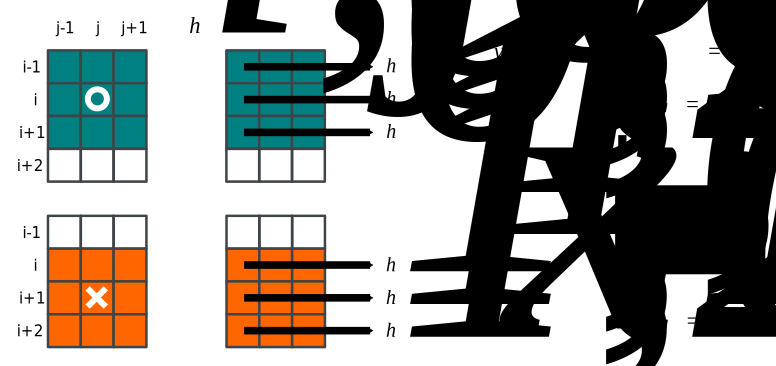
\includegraphics[width=0.55\textwidth]{tiled-conv}
    \caption{Tiled convolution flow}
    \label{pic-tiled-conv}
\end{wrapfigure}


The final step is an optimization published by Advanced Micro Devices (AMD) 
described in \cite{tiled-convolution}. They take advantage from using
separable kernels and reusing operations to get the most out of resources.
We can see separable convolution as a two step process. 
First a horizontal convolution step that creates a set of coefficients 
($h_{y,x}$ in the middle of Fig. \ref{pic-tiled-conv}). Most $h$ coefficients 
are shared by immediate vertical neighbours (e.g. pixels $\hm{\circ}$ 
and $\bm{\times}$ in Fig. \ref{pic-tiled-conv}), thus it is desired 
to reuse them instead of re-computing them. This way, every core in the GPU 
will compute 2 pixels in order to efficiently compute a 2D convolution; plus 
most of this operations are done using registers which is the fastest memory 
available to the cores.


\subsubsection{Comparison}
The Naïve approach seems to be much faster than any other attempts for the 
smallest kernel ($3\times3$), this is simply because a single DoG kernel would
require 9 operations while a separated DoG requires 12. As the size of the
kernels increases tiled convolution has the lead performance-wise.
\begin{table}[hbt]
    \begin{center}
        \caption{Time comparison of different convolution algorithms.}
        \bgroup
        \def\arraystretch{1.2}
        \begin{tabular}{|c|c|c|c|c|}
            \hline Algorithm & Midget Off-centre & Midget On-centre & Parasol Off-centre & Parasol On-centre \\
            \hline Naïve     & 0.000932 s & 0.003150 s & 0.058797 s & N/A\footnote{Unable to fit kernel into constant memory.} \\ 
            \hline Separated & 0.002953 s & 0.005550 s & 0.017261 s & 0.047226 s \\ 
            \hline Tiled     & 0.001947 s & 0.002722 s &  & \\ 
            \hline 
        \end{tabular} 
        \egroup
    \end{center}
\end{table}
\vspace*{-20pt}

For the final implementation we take the best times for every \emph{cell type}
and combine them into a ``convolution'' object under the Python programming language.